\section{Results}
\label{sec:results}
Figure \ref{fig:EMvsMCS} shows the expectation values for the energy and absolute magnetisation as a function of Monte Carlo sweeps with both an ordered and unordered initial configuration. Results for a low temperature 1.0 and a higher temperature 2.4, which is above the critical temperature, are shown. One can see that the expectation values stabilises almost immediately when an ordered starting configuration is chosen for the lower temperature. But when an unordered configuration is chosen, the values does not stabilise until about $25000$ $mcs$. As for the higher temperature, both an ordered and unordered initial configuration gives a result that stabilises quite fast around a value, with some fluctuations. This happens after about 5000 $mcs$ for the energy, and after about 10000 $mcs$ for the magnetisation.   
\begin{figure}[htbp]
	\centering
	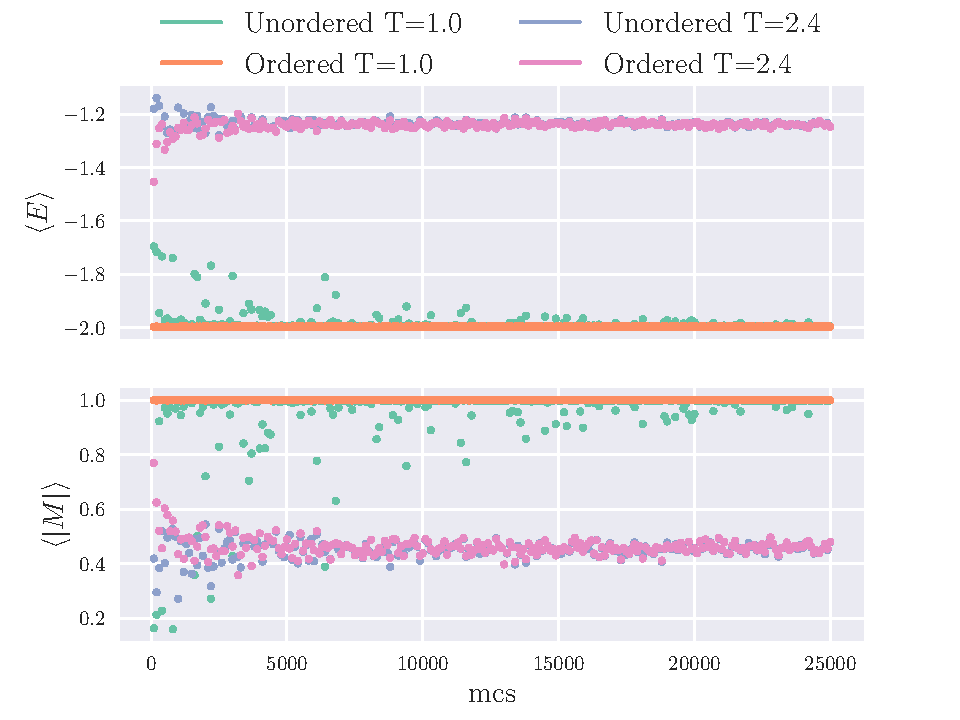
\includegraphics[width=0.5\textwidth]{EMvsMCS.pdf}
	\caption{Plot over expectation values for energy $E$ per spin and absolute magnetisation $|M|$ per spin as a functions of Monte Carlo sweeps $mcs$. The expectation values are plotted for $T=1.0$ and $T=2.4$ with both an ordered and unordered initial state. Lattice size $L=20$ was used.}
	\label{fig:EMvsMCS}
\end{figure}

In Figure \ref{fig:nAccepted}, the number of accepted configurations as a function of Monte Carlo cycles is shown. Again this is plotted for temperatures 1.0 and 2.4, with both an unordered and ordered initial configuration. 

In the case of an ordered initial configuration for the lower temperature, the graph is linear in the logarithmic space, with a slope of about 1. Looking at the graphs for the higher temperature, the same trend can be seen, with the graphs shifted upward a distance of about 1 in log space compared to the lower temperature. For few $mcs$, one can see that the higher temperature graph with an unordered initial configuration lays slightly over the graph for the ordered initial configuration. 

The graph for the lower temperature with an unordered starting configuration starts of with about $10^3$ accepted new configurations for 10 $mcs$, well above the ordered case. From about $10^4$ $mcs$ and out, the two graphs follow each other. 
\begin{figure}[htbp]
	\centering
	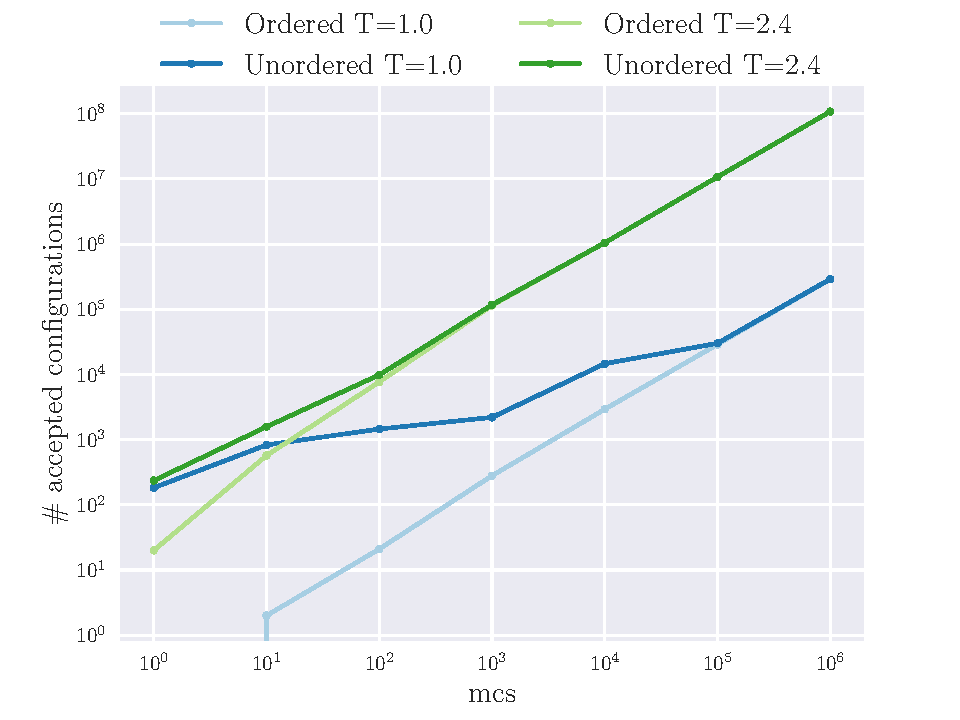
\includegraphics[width=0.5\textwidth]{nAccepted.pdf}
	\caption{Plot over the accumulated number of accepted configurations as a function of Monte Carlo sweeps $mcs$. The number of accepted configurations are plotted for $T=1.0$ and $T=2.4$ with both an ordered and unordered initial state. Lattice size $L=20$ was used. The scale is logarithmic.}
	\label{fig:nAccepted}
\end{figure}

The probability distribution of $E$ per spin is shown in Figure \ref{fig:prob}. For the temperature 1.0 the possible states are all close to -2.0, with two states highly more probable than the others. For the temperature 2.4, the distribution is closer to a normal distribution, with the most probable states around -1.2. The expectation value and variance of $E$ for the same temperatures are shown in Table \ref{tab:prob}.
\begin{figure}[htbp]
	\centering
	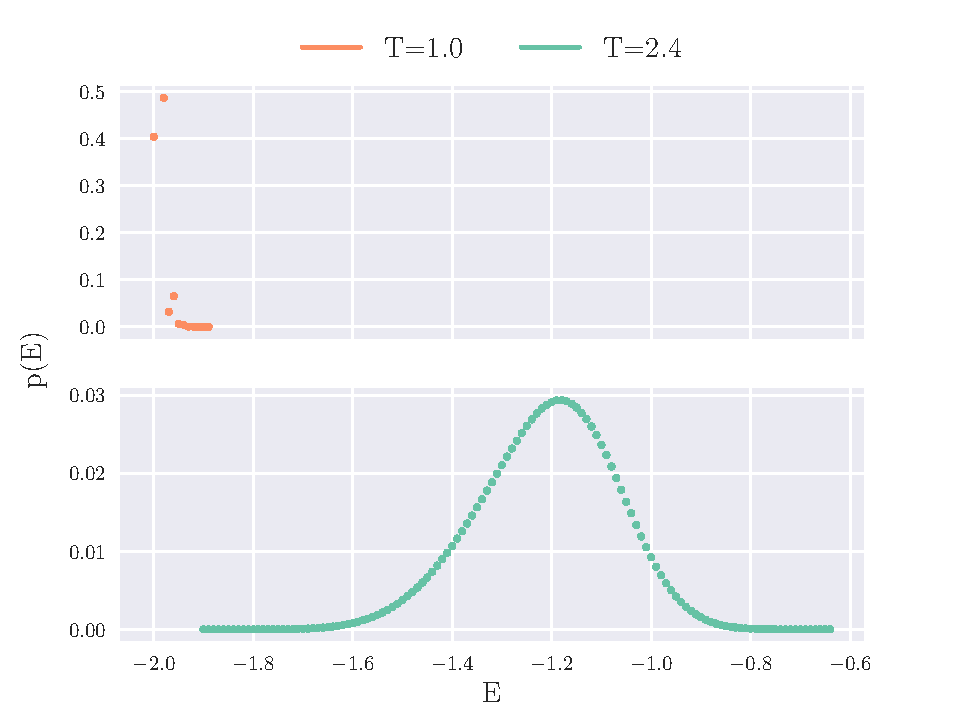
\includegraphics[width=0.5\textwidth]{probability.pdf}
	\caption{Plot over probabilities for a given energy $E$ per spin. The top plot is for temperature $T = 1.0$ while the bottom plot is for temperature $T=2.4$. $10^6$ $mcs$ were used. Lattice size $L=20$ was used.}
	\label{fig:prob}
\end{figure}
\begin{table}[htbp]
	\centering
	\begin{tabular}{lll}
		T   & $\left\langle E\right\rangle$  & $\sigma^2$ \\
		\hline
		\addlinespace[0.1cm]
		1.0   & -1.997 & 0.025 \\
		2.4 & -1.237  & 8.116
	\end{tabular}
	\caption{Table over the expectation value  $\left\langle E\right\rangle$ and variation  $\sigma^2$ of the energy per spin after $10^6$ $mcs$ for temperatures $T=1.0$ and $T=2.4$. Lattice size $L=20$ was used.}
	\label{tab:prob}
\end{table}

Figure \ref{fig:E} and \ref{fig:M} shows the expectation values for the energy and the absolute magnetisation from $T=2.0$ to $T=2.3$, while Figure \ref{fig:C} and \ref{fig:Chi} shows the specific heat and susceptibility for the same temperature interval. In all these plots results for lattices with size $L=40,60,80$ and 100 are shown. 

In the energy plot, all expectation values are negative, and increases as temperature increase. For temperatures under 2.25, all the lattices gives the same results, but for higher temperatures, the values slightly diverge from each other.
 
A similar trend is found in the plot of the absolute magnetisation. The values for the different lattices are very similar until a temperature of about 2.20, and then diverge. Comparing the energy and magnetisation plots, the magnetisation values diverge more strongly from each other. All the magnetisation values are positive, and decrease as the temperature increases.   

The plots over the specific heat and the susceptibility does also feature a divergent trend in the temperature interval 2.20 to 2.30. In addition, the plots are less smooth in this interval. The specific heat values increase with temperature until they reach a maxima between 2.25 and 2.30. The maximum values are slightly shifted towards lower temperatures as L increase. In the susceptibility plot, only the results for the lattice size $L=100$ has a maxima in this interval.  
\begin{figure}[htbp]
	\centering
	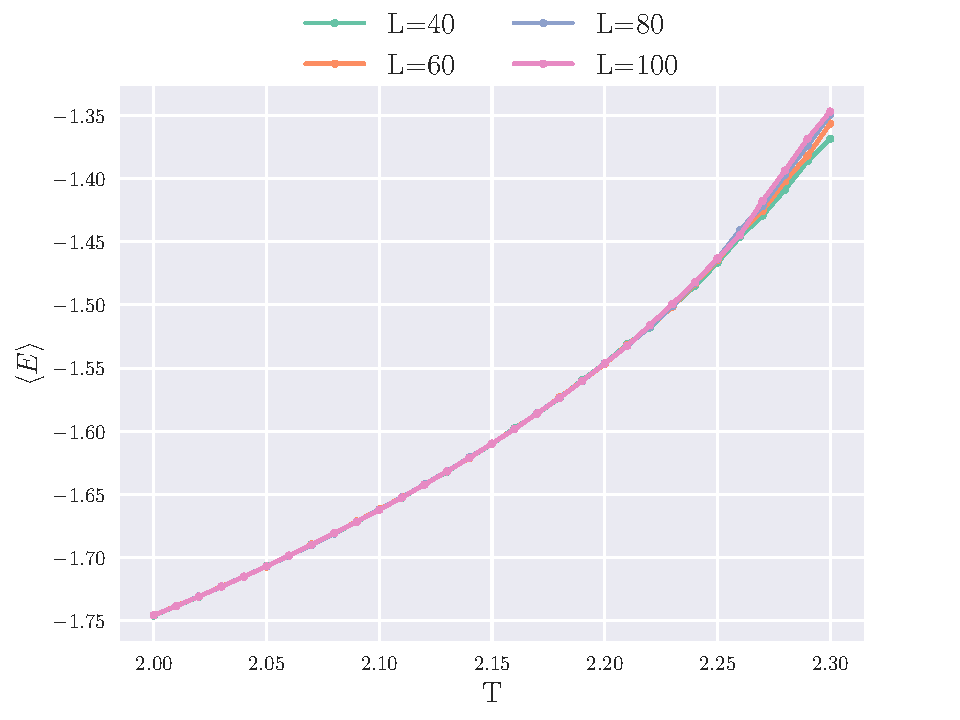
\includegraphics[width=0.5\textwidth]{energy.pdf}
	\caption{Plot over the expectation values for the energy per spin $\left\langle E\right\rangle$ as a function of temperature $T$ with step size $10^{-3}$. The results are from lattices with size $L=40,60,80$ and 100.  $10^6$ $mcs$ were used for each step.}
	\label{fig:E}
\end{figure}

\begin{figure}[htbp]
	\centering
	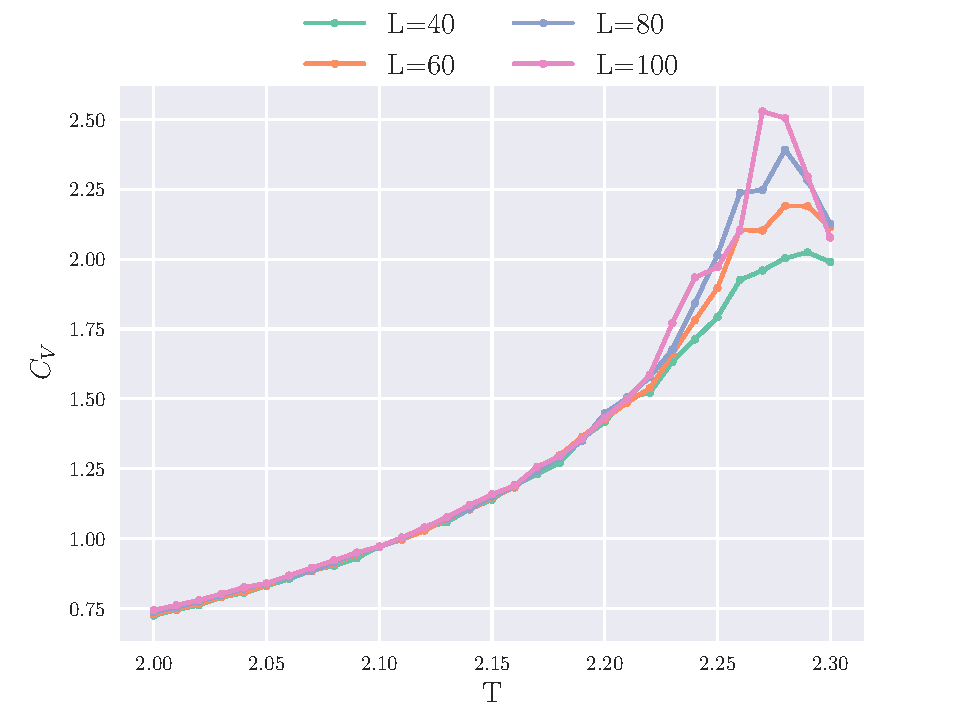
\includegraphics[width=0.5\textwidth]{heat_capacity.pdf}
	\caption{Plot over the expectation valuess for the specific heat per spin $C_V$ as a function of temperature $T$ with step size $10^{-3}$. The results are from lattices with size $L=40,60,80$ and 100. $10^6$ $mcs$ were used for each step.}
	\label{fig:C}
\end{figure}

\begin{figure}[htbp]
	\centering
	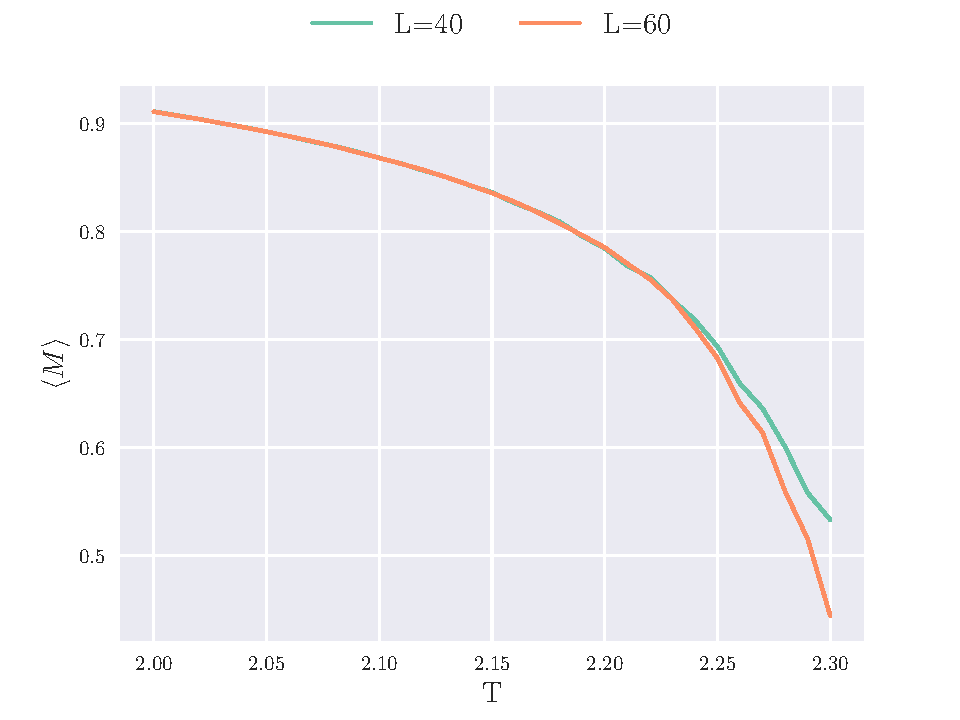
\includegraphics[width=0.5\textwidth]{magnetization.pdf}
	\caption{Plot over the expectation value for the absolute magnetisation per spin $\left\langle |M|\right\rangle$ as a function of temperature $T$ with step size $10^{-3}$. The results are from lattices with size $L=40,60,80$ and 100. $10^6$ $mcs$ were used for each step.}
	\label{fig:M}
\end{figure}

\begin{figure}[htbp]
	\centering
	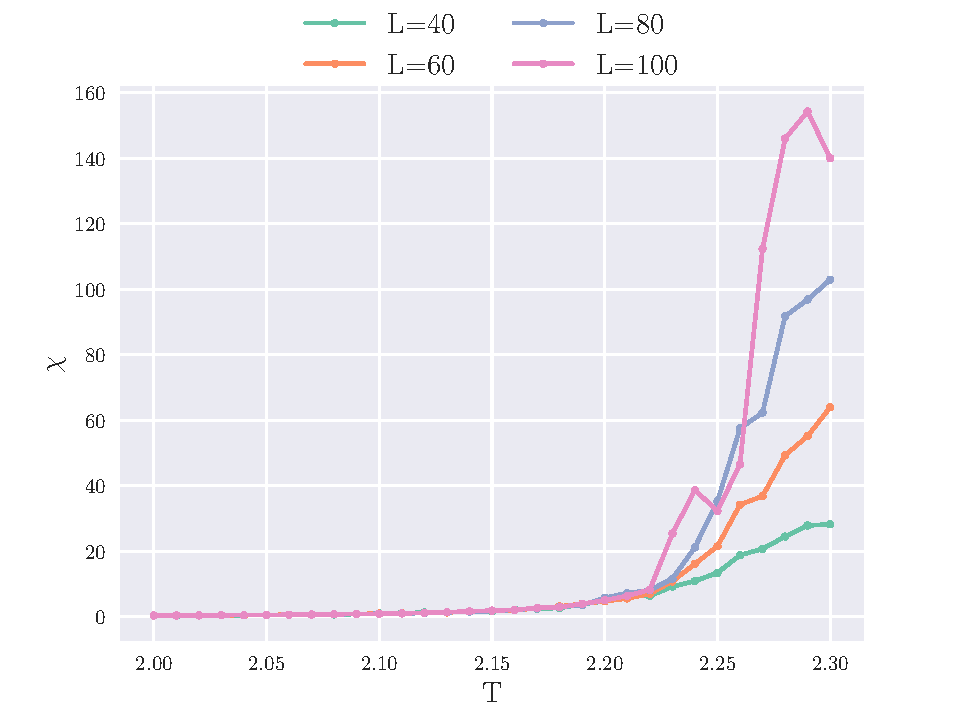
\includegraphics[width=0.5\textwidth]{susceptibility.pdf}
	\caption{Plot over the expectation values for the susceptibility per spin $\chi$ as a function of temperature $T$ with step size $10^{-3}$.The results are from lattices with size $L=40,60,80$ and 100. $10^6$ $mcs$ were used for each step.}
	\label{fig:Chi}
\end{figure}

Figure \ref{fig:zoom} shows results for the specific heat in the temperature interval 2.26 to 2.30 with a higher resolution than Figure \ref{fig:C}. In addition, a running mean is shown.  
\begin{figure}[htbp]
	\centering
	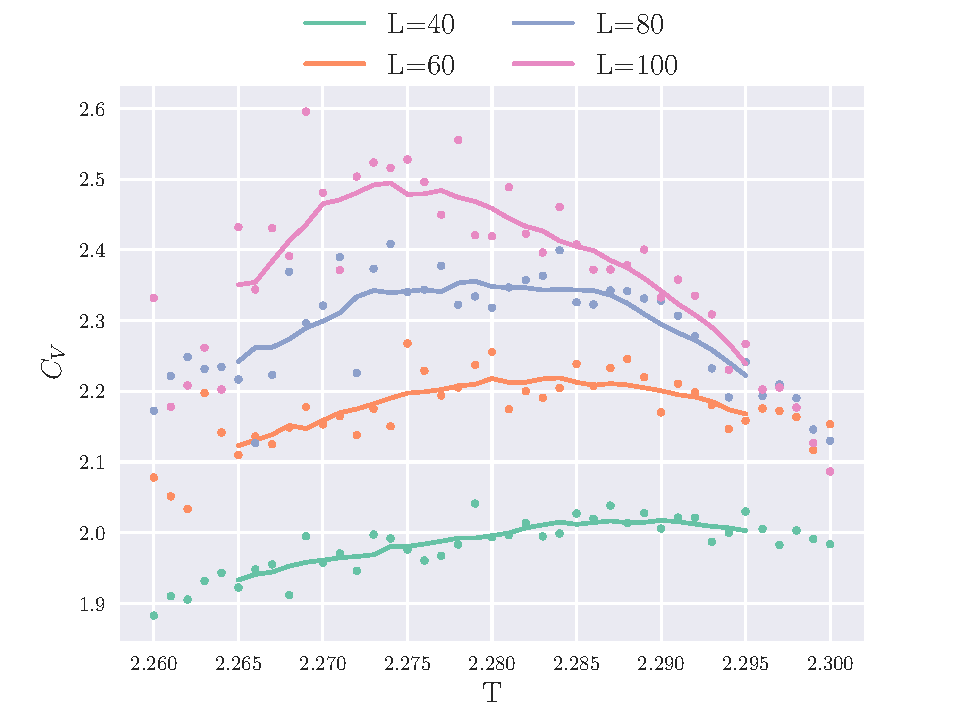
\includegraphics[width=0.5\textwidth]{zoom.pdf}
	\caption{Plot over the expectation values for the specific heat per spin $C_V$ as a function of temperature $T$ with step size $10^{-4}$.The results are from lattices with size $L=40,60,80$ and 100. $10^6$ $mcs$ were used for each step. The dots are the collected data, while the solid line is a running mean with a window size of 11.}
	\label{fig:zoom}
\end{figure}

Table \ref{tab:Tc} lists the calculated values for the critical temperature $T_c$ in the thermodynamic limit $L \rightarrow \infty$  using the data shown in Figure \ref{fig:C} and \ref{fig:zoom}. One can see that all means are within one standard deviation from the analytical value. The higher resolution data set (Figure \ref{fig:zoom}) gives a mean value closer to the analytical value. There mean value of the results using a running mean is the same as when no running mean is applied. 
\begin{table}[]
	\centering
	\begin{tabular}{rrrrr}
		$L_i$         & $L_j$ & LR  & HR & HRRM \\
		\hline
		\addlinespace[0.1cm]
		60            & 40    & 2.260 & 2.267 & 2.272     \\
		80            & 40    & 2.270 & 2.269 & 2.268     \\
		80            & 60    & 2.280 & 2.271 & 2.264     \\
		100           & 40    & 2.257 & 2.262 & 2.263     \\
		100           & 60    & 2.255 & 2.260 & 2.259     \\
		100           & 80    & 2.230 & 2.249 & 2.254     \\
		\hline
		\addlinespace[0.1cm]
		\textbf{Mean} &       & 2.259 & 2.263 & 2.263     \\
		\textbf{STD}  &       & 0.015 & 0.007 & 0.006    
	\end{tabular}
	\caption{Critical temperature in the thermodynamic limit $L \rightarrow \infty$ calculated using eq. \ref{eq:Tc} for different lattice sizes $L$. Results using low resolution values (LR) plotted in Figure \ref{fig:C}, high resolution values (HR) and the running mean of the high resolution values (HRRM) plotted in Figure \ref{fig:zoom} are shown. In addition, the mean value and standard deviation (STD) for each set of values are shown.}
	\label{tab:Tc}
\end{table}
